\chapter{Cheat Features Implemented in Our Cheat for CS2}

This chapter provides a comprehensive analysis of the \textbf{cheat features} we have successfully implemented within our \textit{cheat}. We will explore their objectives, the underlying logic governing their operation, and the technical implementation that enables them to function correctly. Each section will present \textbf{code snippets} that illustrate key parts of our implementation, allowing for a deeper understanding of how we interfaced with the CS2 engine. Furthermore, we will outline the specific \textbf{functions we have hooked}, demonstrating how we gain control over critical game processes to manipulate rendering, aiming, and other essential aspects of gameplay.


\begin{table}[h]
    \centering
    \renewcommand{\arraystretch}{1.3} % Improves row spacing
    \setlength{\tabcolsep}{6pt} % Adjust column spacing to fit better
    \resizebox{\textwidth}{!}{ % Resize table to fit within page width
    \begin{tabular}{@{} l p{9cm} @{}}
        \toprule
        \textbf{Functionality} & \textbf{Description} \\
        \midrule
        \textbf{Chams} & Modifies the rendering pipeline to apply custom materials to in-game models, enhancing visibility. \\
        \textbf{ESP (Extra Sensory Perception)} & Extracts and displays real-time enemy information, providing a tactical advantage. \\
        \textbf{Aimbot} & Automates aiming mechanisms to improve accuracy and precision. \\
        \textbf{Anti-Aim} & Manipulates player model orientation to mislead enemy aimbots and disrupt targeting. \\
        \bottomrule
    \end{tabular}
    }
    \caption{Core Functionalities Overview}
    \label{tab:core_functionalities}
\end{table}






There exist multiple approaches to implementing each of these cheat features, ranging from simple external overlays to deep internal hooks that modify game memory and execution flow. Given the time constraints of this work and the limited publicly available documentation on cheat development, we have opted for an approach that provides the best balance between effectiveness and stealth. 

The lack of official documentation and the inherently secretive nature of cheat development meant that much of our implementation had to be based on reverse engineering and extensive experimentation. Instead of relying on external overlays, which are more susceptible to detection and performance limitations, or resorting to aggressive memory manipulation, which significantly increases the risk of being flagged by anti-cheat systems, we chose to integrate directly with the game’s internal systems. 


We begin by exploring \textbf{Chams}, one of the most visually impactful modifications. This technique alters the appearance of in-game models by replacing their default materials with custom ones, effectively enhancing player visibility. Unlike traditional \textit{ESP} methods, which rely on external overlays that merely draw information on the player’s screen, Chams modify the rendering process within the engine itself. This allows for an entirely integrated solution that operates without any \textbf{performance impact}, making it one of the most effective and undetectable visual enhancements available. 

In the following sections, we will dissect the logic behind our Chams implementation, detailing how we intercept key rendering functions, modify material properties, and dynamically apply custom textures to selected in-game entities. Each aspect of the implementation will be supported by relevant code snippets, providing an in-depth look at how we have programmed this feature.


\section{Chams: Enhancing Visibility Through Engine-Based Rendering}
Chams (\textit{chameleon skins}) is a rendering manipulation technique that enables the replacement of standard in-game materials with custom-designed ones, significantly enhancing model visibility and allowing players to track enemy movements with greater ease regardless of lighting conditions, distance, or obstacles that would typically obscure their position. 

Unlike external overlays, which function independently from the game and merely display additional information on the screen, Chams operate directly within the game engine, modifying the rendering logic at its core to ensure seamless integration and optimal performance without introducing additional processing overhead. 

By leveraging hooking techniques within CS2’s material system, it becomes possible to dynamically inject new textures and visual effects that are not present in the base game, allowing for a level of customization that surpasses conventional graphical modifications while maintaining the efficiency and fluidity of the rendering pipeline.

To achieve this level of modification, we implemented a multi-step process that ensures full integration with the game's rendering system. This process consists of the following key components:

\begin{itemize}
    \item \textbf{Extracting Default Materials from the Game Engine} – Understanding and retrieving the default materials used by the game.
    \item \textbf{Generating Custom Materials} – Creating and defining new textures and visual effects that will replace the existing materials.
    \item \textbf{Hooking CreateMaterial and Injecting Custom Materials} – Intercepting the game's material creation functions to replace default materials with our customized versions dynamically.
    \item \textbf{Hooking OnDrawModelExecute and Overriding Materials} – Modifying the rendering function responsible for drawing models to enforce the application of custom materials in real-time.
\end{itemize}

In the following sections, we will provide a detailed explanation of each of these steps, outlining how they contribute to the seamless integration of Chams into the CS2 rendering pipeline. We will delve into the technical specifics of how default materials are extracted, how custom materials are generated, and how we hook into the rendering functions to ensure that these modifications persist across all game instances.



\subsection{Extracting Default Materials from the Game Engine}

To fully understand how materials are structured and applied in CS2, we conducted extensive \textbf{debugging of the rendering engine}. By hooking into the \textbf{OnDraw} function, we intercepted the material creation process and successfully extracted the data of a default in-game material.

The following is an example of a material retrieved directly from the CS2 engine:

\begin{lstlisting}[style=cppstyle, caption={Extracted Default Material from CS2}]
<!-- kv3 encoding:text:version{e21c7f3c-8a33-41c5-9977-a76d3a32aa0d}
    format:generic:version{7412167c-06e9-4698-aff2-e63eb59037e7} -->
    {
        shader = "csgo_effects.vfx"
        g_tColor = resource:"materials/dev/primary_white_color_tga_21186c76.vtex"
        g_tNormal = resource:"materials/default/default_normal_tga_7652cb.vtex"
        g_flColorBoost = 30
        g_flOpacityScale = 245.55
        g_vColorTint = [7.0, 7.0, 7.0, 0.37522]
    }
\end{lstlisting}

The extracted material follows the KV3 format, a modernized data structure introduced in Source 2 to replace the older KeyValues system used in Source 1. 

KV3 allows for efficient serialization of structured data, supporting hierarchical organization and multiple data types, making it ideal for defining game assets such as materials, models, and particle effects. The Source 2 engine interprets these material definitions at runtime, applying the specified shader, texture maps, and rendering properties dynamically. By understanding this format, we gain full control over how materials are created and manipulated in CS2, enabling us to inject entirely new visual elements into the game without modifying pre-existing assets.

Further exploration of this format, along with an in-depth analysis of its structure and applications, was possible by studying the official Source 2 Developer Wiki, which provides extensive documentation on how Source 2 processes materials, shaders, and other graphical assets. This resource offered crucial insights into how KV3 interacts with the rendering engine, particularly in the way materials are compiled and utilized in real time.

By modifying this format, we successfully generated a variety of new materials, each possessing unique properties suited for different visual effects, allowing us to experiment with different rendering techniques and further refine our implementation of Chams in CS2.

\subsection{Generating Custom Materials}

After extracting and analyzing a default material from the game, we proceeded to experiment with different configurations to generate a collection of materials optimized for various Chams effects.

The goal of this process was to develop materials capable of altering in-game visibility while maintaining the integrity of CS2’s rendering engine. By modifying specific attributes such as \texttt{g\_flFresnelExponent} for light reflection, \texttt{g\_flOpacityScale} for transparency, and the blending mode flags, we achieved a variety of effects including glow effects, metallic reflections, and enhanced visibility through obstacles.

\begin{lstlisting}[style=cppstyle, caption={List of Custom Materials}]
std::vector <const char *> MaterialInfo = { 
    szVMatBufferWhiteVisible,    szVMatBufferWhiteInvisible,
    szVMatBufferIlluminateVisible,    szVMatBufferIlluminateInvisible,
    szVMatBufferIlatex,        szVMatBufferIlatexInvisible,
    szVMatBufferMetalic,        szVMatBufferMetalicInvisible,
    szVMatBufferGlowVisible,    szVMatBufferGlowInvisible
};
\end{lstlisting}

Each of these materials was assigned a name that reflects its primary visual characteristic to facilitate its integration into our cheat system. By storing these materials in a \textbf{hashmap}, we enable efficient retrieval and reuse whenever new materials need to be applied. 

Since materials in CS2 are defined as structured strings that determine their rendering properties, we ensure that our injected materials adhere to this format. This allows us to seamlessly integrate custom materials into the game's rendering pipeline by hooking into the \texttt{CreateMaterial} function and dynamically replacing standard materials with our own.



One of the most visually distinctive materials we developed was the \textbf{Glow Illuminated} effect. This material was designed to create a glowing outline around player models by leveraging CS2’s built-in material masks and fine-tuning fresnel-based lighting parameters. The final definition of this material is shown below:

\begin{lstlisting}[style=cppstyle, caption={Glow Illuminated Material Definition}] 
static static constexpr char szVMatBufferGlow2Visible[] =
R(<!-- kv3 encoding:text:version{e21c7f3c-8a33-41c5-9977-a76d3a32aa0d}format:generic:version{7412167c-06e9-4698-aff2-e63eb59037e7} -->
    {
        shader = "csgo_effects.vfx"
        g_tColor = resource:"materials/dev/primary_white_color_tga_21186c76.vtex"
        g_tNormal = resource:"materials/default/default_normal_tga_7652cb.vtex"
        g_tMask1 = resource:"materials/default/default_mask_tga_344101f8.vtex"
        g_tMask2 = resource:"materials/default/default_mask_tga_344101f8.vtex"
        g_tMask3 = resource:"materials/default/default_mask_tga_344101f8.vtex"
        g_flOpacityScale = 0.45
        g_flFresnelExponent = 0.75
        g_flFresnelFalloff = 1
        g_flFresnelMax = 0.0
        g_flFresnelMin = 1
        F_ADDITIVE_BLEND = 1
        F_BLEND_MODE = 1	
        F_TRANSLUCENT = 1
        F_IGNOREZ = 0
        F_DISABLE_Z_WRITE = 0
        F_DISABLE_Z_BUFFERING = 0
        F_RENDER_BACKFACES = 1
        g_vColorTint = [1.0, 1.0, 1.0, 0.0]
});
\end{lstlisting}


This configuration takes advantage of Source 2’s built-in rendering properties to produce a highly effective glow effect. The fresnel parameters control how light interacts with the surface, ensuring that the glow intensity changes dynamically based on the player's viewing angle. Additionally, the use of multiple texture masks helps the glow blend naturally into the surrounding environment, making it appear as a seamless part of the game's visual style rather than an artificial overlay.

By refining these materials through iterative testing and real-time observation, we successfully developed a collection of custom visual effects that seamlessly integrate into CS2’s rendering engine. This process not only allowed us to enhance player visibility but also provided deeper insights into the flexibility of Source 2’s material system. The ability to dynamically inject and apply new materials in real time offers significant advantages, as it enables rapid adjustments to the cheat’s visual effects without requiring modifications to game files or precompiled assets.

Through the careful selection of material properties and the precise manipulation of CS2’s rendering functions, we have created a system that allows for highly customizable visual enhancements. These materials serve as the foundation for our Chams implementation, which will be further detailed in the following sections.


\subsection{Hooking CreateMaterial and Injecting Custom Materials}

To dynamically create and register materials in CS2, we hooked into the \textbf{CreateMaterialFunction}, allowing us to manipulate how the game initializes and stores materials.

\begin{lstlisting}[style=cppstyle, caption={Hooking CreateMaterial Function}]
static int64_t (__fastcall *CreateMaterialFunction)(void *, void *, const char *, void *, unsigned int, unsigned int);
\end{lstlisting}

With this function, we dynamically generated and injected new materials into the game:

\begin{lstlisting}[style=cppstyle, caption={Creating a Custom Material in Memory}]
CMaterial2 *CreateCustomMaterial(const char *materialName, const char *materialData) {
    CKeyValues3 *pKeyValues = CreateMaterialResource();
    if (!pKeyValues) return nullptr;

    LoadKeyValues(pKeyValues, nullptr, materialData, nullptr, nullptr, nullptr, nullptr, nullptr, "");
    CMaterial2 *customMaterial = nullptr;
    CreateMaterialFunction(nullptr, &customMaterial, materialName, pKeyValues, 0, 1);
    return customMaterial;
}
\end{lstlisting}

\subsection{Loading KV3 Materials into the Game}  

After defining the custom materials, they must be properly loaded into the game engine so that they can be recognized and applied during rendering. This process involves parsing the KV3 data and ensuring that the Source 2 engine interprets it correctly. Without this step, the materials would remain as raw data in memory and would not be accessible for rendering operations. The following function is responsible for handling this process:  

\begin{lstlisting}[style=cppstyle, caption={Loading a KV3 Material into the Game}]
bool Visual::Chams::LoadKV3 (CUtilsBuff *buff, CKeyValues3 *CkeyVal) 
{
    KV3ID_t kv3ID = KV3ID_t ("generic", 0x41B818518343427E, 0xB5F447C23C0CDF8C);
    return LoadKeyValues (CkeyVal, nullptr, buff, &kv3ID, nullptr, nullptr, nullptr, nullptr, "");
}
\end{lstlisting}  

This function plays a critical role in ensuring that the Source 2 engine correctly processes and integrates the KV3 material data. The most notable aspect of this function is the initialization of the \texttt{KV3ID\_t} object, which serves as a unique identifier for the KV3 data format. The string \texttt{"generic"} suggests that the format follows a standard KV3 structure. However, the most crucial part of this initialization lies in the two hexadecimal values: \texttt{0x41B818518343427E} and \texttt{0xB5F447C23C0CDF8C}.  

These identifiers are likely used by the Source 2 engine as a reference signature for processing specific types of KV3 data. The first hexadecimal value, \texttt{0x41B818518343427E}, may act as a format validation key that the engine checks to ensure that the data being loaded conforms to the expected KV3 structure. The second identifier, \texttt{0xB5F447C23C0CDF8C}, could correspond to a particular category of KV3 files, distinguishing different types of resource files such as materials, models, or particle effects. This mechanism prevents malformed or incompatible KV3 data from being processed, ensuring that only correctly structured material definitions are registered in the engine.  

Once the KV3 identifier is established, the function calls \texttt{LoadKeyValues}, which processes the KV3 data stored in memory. This function takes the parsed key-value pairs, ensures that the format aligns with the engine's expectations, and then integrates the material into the game’s resource management system. The function parameters include a reference to the parsed data, a pointer to the KV3 identifier, and several \texttt{nullptr} arguments, which indicate that no additional optional parameters are required in this context.  

By executing this function, the Source 2 engine successfully processes and registers the material, making it available for rendering in real-time. The use of predefined hexadecimal identifiers ensures that the KV3 data is correctly formatted and compatible with the rendering system. This approach enables the dynamic application of custom materials, allowing for real-time modifications without requiring precompiled assets or modifications to the game’s existing files. The ability to inject materials dynamically provides a powerful method for implementing features such as Chams, enhanced weapon skins, and other visual modifications while maintaining full compatibility with the game engine.




\subsection{Hooking \texttt{OnDrawModelExecute} and Overriding Materials}

To dynamically apply Chams, we intercepted \texttt{OnDrawModelExecute}, the function responsible for rendering in-game models. By hooking into this function, we gained control over the rendering process, allowing us to selectively modify materials applied to specific in-game entities. This method ensures that our custom materials are seamlessly integrated into the game's rendering pipeline without introducing additional rendering overhead or external overlays.

\subsubsection{Filtering Target Entities}

Since \texttt{OnDrawModelExecute} processes all rendered models, it is necessary to implement a filtering mechanism to ensure that only relevant entities—such as enemy players and weapons—are affected by our Chams system. Without this step, the modification would be applied indiscriminately to all objects in the game, including environmental elements and friendly players, which is neither efficient nor desirable.

To achieve this, we retrieve the schema name of each entity and compare it against known identifiers for player models and weapons. For player models, we check whether the entity corresponds to a \texttt{C\_CSPlayerPawnBase} instance, which represents in-game characters.

\begin{lstlisting}[style=cppstyle, caption={Identifying Player Models}]
auto schemaName = iGameEntitySystem->GetSchemaName(pEntity);
if (strcmp(schemaName.c_str(), "C_CSPlayerPawnBase") == 0) {
    applyCustomMaterial(pMesh);
}
\end{lstlisting}

Similarly, for weapons, we filter out entities corresponding to \texttt{C\_PredictedViewModel}, ensuring that Chams are also applied to the player's held weapon model.

\begin{lstlisting}[style=cppstyle, caption={Applying Chams to Weapons}]
if (strcmp(schemaName.c_str(), "C_PredictedViewModel") == 0) {
    applyCustomMaterial(pMesh, weaponMaterial);
}
\end{lstlisting}

By implementing this filtering mechanism, we ensure that Chams are applied exclusively to relevant gameplay elements, enhancing player visibility without interfering with other rendered objects.

\subsubsection{Overriding Material Pointers}

Once the relevant entities are identified, the next step is to override their assigned materials with our custom Chams textures. This is achieved by modifying the material pointer associated with the target model.

\begin{lstlisting}[style=cppstyle, caption={Overriding Model Materials}]
arrMeshDraw->CMaterial = *(CMaterial2 **)CustomMaterialMap.at(MaterialName);
\end{lstlisting}

This modification dynamically replaces the original material with one of our preloaded Chams materials stored within the \texttt{CustomMaterialMap}. By performing this override at runtime, we ensure that our changes take effect immediately, without requiring any modification to the game's original assets. This approach enables real-time visual adjustments and allows for the implementation of different Chams effects based on user preferences or situational requirements.

By leveraging this hooking technique, we achieve a stealthy and efficient modification of the rendering pipeline, integrating custom materials in a way that is indistinguishable from the game's native rendering behavior. This method not only enhances the effectiveness of Chams but also serves as a foundation for further graphical modifications within the cheat system.


\begin{figure}[h!]
    \centering
    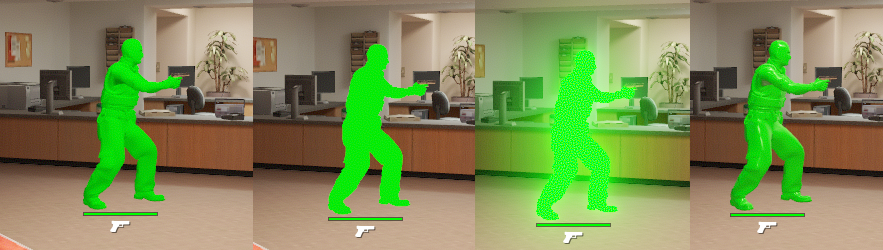
\includegraphics[width=1\linewidth]{images/ZqBsYBx.png}
    \caption{Created Chams Materials}
    \label{fig:enter-label}
\end{figure}

\subsubsection{Visible vs Non-Visible Chams Logic}

Once this logic is in place, we can take it a step further and assign different materials to the visible and non-visible parts of the enemy player model. This allows us to render, for example, the visible part of the player in one color (e.g., purple) and the non-visible part (e.g., behind walls) in another (e.g., yellow). 

Since this rendering is only visible locally to the cheat user and not to other players in the match, it enables us to appear as a legitimate player with significantly better awareness and reflexes. By clearly seeing which parts of an enemy are exposed and which are not, we can ensure to only target the visible areas.

This reduces the risk of suspicious-looking shots (such as pre-firing through walls or headshots through solid cover) and helps us maintain a "legit" playstyle that blends in with skilled human behavior. In turn, this greatly decreases the chances of triggering manual bans during demo reviews or overwatch-like systems, where human moderators could flag unnatural behavior.


\begin{figure}
    \centering
    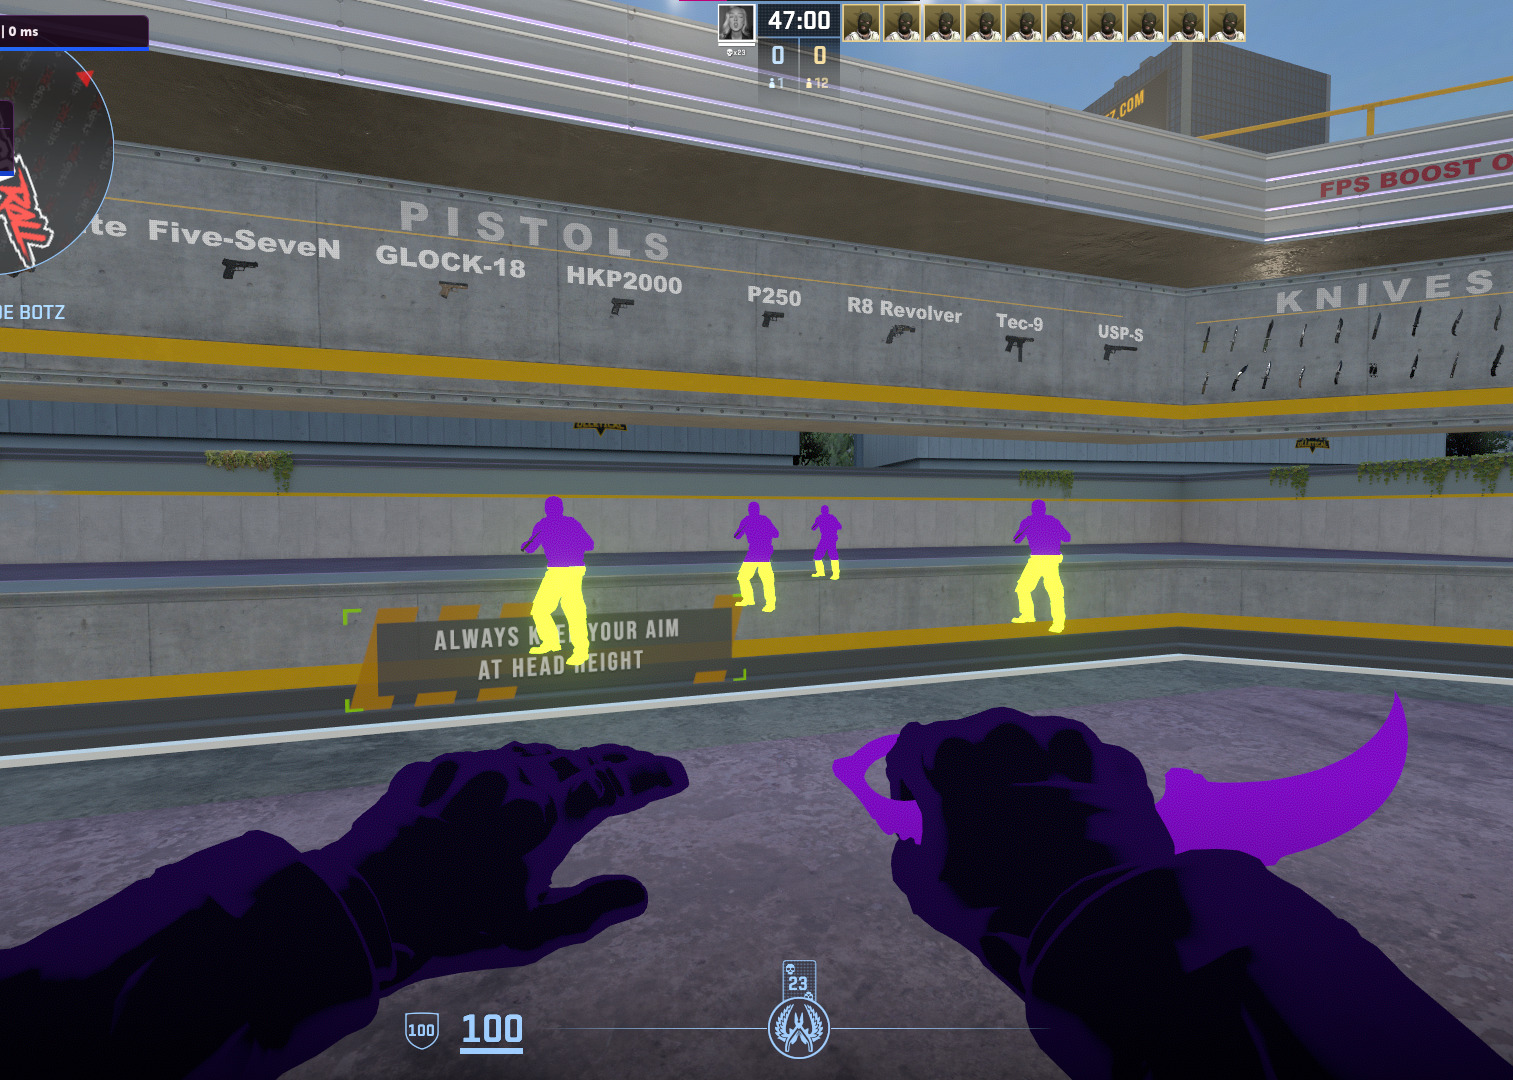
\includegraphics[width=1\linewidth]{images/visible_invisible_chams.png}
    \caption{Enter Caption}
    \label{fig:enter-label}
\end{figure}


\newpage


\section{Aimbot: Automated Aim to Enemy Players}


An aimbot is one of the most fundamental and widely recognized cheat functionalities in competitive first-person shooters. It automates the aiming process by computing the precise trajectory required to target an enemy, thereby bypassing human limitations in reaction time and accuracy. Developing an aimbot for \textit{Counter-Strike 2} (CS2) necessitates a comprehensive understanding of the game’s \textbf{entity system}, \textbf{coordinate transformations}, and \textbf{trigonometric principles} to ensure precise target alignment.

However, before implementing the aiming mechanism, it was crucial to first analyze how CS2 internally manages game entities. This understanding was essential since retrieving a player's position and calculating the required angles for the aimbot depend on accessing valid entity data. Without proper entity management, attempting to access a non-existent player could lead to dereferencing null pointers, resulting in critical errors or crashes.



\subsection{Entity Management: Hooking the Game's Entity System}

CS2 maintains an internal \textbf{entity system} that is responsible for handling all game objects, including players. Each entity is uniquely identified and assigned a memory address, allowing the game to track its state efficiently. Unlike other dynamic game objects that are continuously updated, player entities in CS2 follow a more static lifecycle: they are loaded into memory once a player connects to a server and remain persistent unless a player disconnects or a new player joins the match. This means that, unlike projectiles or temporary objects, player entities are only modified under specific conditions, reducing unnecessary updates and improving performance.

To reliably access player data and maintain an up-to-date reference to all active players, we identified and hooked into two critical functions within the game's entity management system:

\begin{itemize}
    \item \textbf{OnAddEntity} – Responsible for adding new entities to the game. When a player joins a match, the game dynamically allocates memory for a new entity, assigns it a unique identifier, and registers it in the entity system.
    \item \textbf{OnRemoveEntity} – Handles the cleanup and removal of entities when they leave the match. When a player disconnects or is kicked, the entity system marks their associated entity for deletion and releases the allocated memory.
\end{itemize}

By intercepting these functions, we effectively track player entities and store their references in a \textbf{hashmap}. This hashmap allows us to maintain real-time access to entity data while preventing invalid memory access. Since player entities are only modified when a new player joins or an existing player disconnects, the hashmap remains stable and does not require frequent updates, unlike entity lists that need to be re-queried every frame.

We implemented hooks for \texttt{OnAddEntity} and \texttt{OnRemoveEntity} to ensure our entity tracking remains consistent throughout a match. By leveraging \textbf{hashmaps}, we can efficiently store and retrieve player-related entities, reducing overhead and ensuring a seamless interaction with the game's entity system. Furthermore, this approach minimizes reliance on manually finding offsets, as entity references remain valid until explicitly removed by the engine.



\begin{lstlisting}[style=cppstyle, caption={OnAddEntity Hook}]
void HooksManager::OnAddEntity::hOnAddEntity(__int64 CGameEntitySystem, void *entityPointer, int entityHandle) {
    oOnAddEntity(CGameEntitySystem, entityPointer, entityHandle);

    if (strcmp(iGameEntitySystem->GetSchemaName(entityPointer).c_str(), "C_CSPlayerPawnBase") == 0) {
        iGameEntitySystem->PawnMap.insert(std::make_pair(entityHandle, (C_PlayerPawn *)entityPointer));
    }
    if (strcmp(iGameEntitySystem->GetSchemaName(entityPointer).c_str(), "CBasePlayerController") == 0) {
        iGameEntitySystem->ControllerMap.insert(std::make_pair(entityHandle, (C_PlayerController *)entityPointer));
    }
}
\end{lstlisting}

\begin{lstlisting}[style=cppstyle, caption={OnRemoveEntity Hook}]
void HooksManager::OnRemoveEntity::hOnRemoveEntity(__int64 CGameEntitySystem, void *entityPointer, int entityHandle) {
    oOnRemoveEntity(CGameEntitySystem, entityPointer, entityHandle);

    if (strcmp(iGameEntitySystem->GetSchemaName(entityPointer).c_str(), "C_CSPlayerPawnBase") == 0) {
        iGameEntitySystem->PawnMap.erase(entityHandle);
    }
    if (strcmp(iGameEntitySystem->GetSchemaName(entityPointer).c_str(), "CBasePlayerController") == 0) {
        iGameEntitySystem->ControllerMap.erase(entityHandle);
    }
}
\end{lstlisting}


By correctly associating players with their respective controller and pawn structures, we ensure that all entity references remain valid.


\subsubsection{Computing Aiming Angles}

Achieving precise aiming in a three-dimensional environment like \textit{Counter-Strike 2} requires the aimbot to compute angular adjustments that align the player's crosshair with a target. Player orientation in CS2 is defined by three rotational angles:

\begin{itemize}
    \item \textbf{Pitch} (\(\theta\)): Controls vertical movement, determining how much the player looks up or down.
    \item \textbf{Yaw} (\(\phi\)): Governs horizontal movement, rotating the player's view left or right.
    \item \textbf{Roll} (\(\psi\)): Represents tilt along the forward axis but remains fixed at zero in CS2.
\end{itemize}

\begin{figure}[h!]
    \centering
    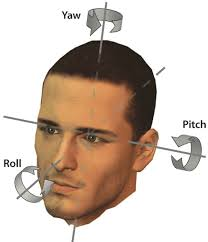
\includegraphics[width=0.4\linewidth]{images/image.png}
    \caption{Representation of Pitch, Yaw, and Roll in a 3D Space.}
    \label{fig:pitch_yaw_roll}
\end{figure}

While \textbf{pitch} and \textbf{yaw} dictate aiming direction in CS2, the \textbf{roll angle} remains fixed at zero. Unlike flight simulators or VR applications, where roll introduces an additional degree of freedom, CS2 enforces strict constraints that prevent camera tilting. Altering the roll angle would lead to an \textbf{impossible in-game state}, triggering \textbf{Valve Anti-Cheat (VAC)} detection and an automatic ban.



\subsubsection{Deriving the Direction Vector}

To accurately compute the aiming angles, the first step is to determine the enemy's position relative to the player's viewpoint. This process involves obtaining the player's position on the map, referred to as the \emph{foot position}, and then retrieving the camera position, which represents the player's \emph{eye position}. The eye position is the viewpoint from which the player perceives the game environment.

All positions are represented as three-dimensional vectors, \( \text{Vec3} \), consisting of three floating-point values: \( x, y, z \).

\subsubsection{Computing the Player’s Position}

The player's final position in the game world is obtained by adding the base position of the player to the camera offset:

\[
P_{\text{player}} = P_{\text{base}} + P_{\text{camera}}
\]

Where:
\begin{itemize}
    \item \( P_{\text{player}} \) is the final computed position of the player.
    \item \( P_{\text{base}} \) is the player's base position in the world.
    \item \( P_{\text{camera}} \) is the camera offset (view position).
\end{itemize}

Expressed in vector form:

\[
\mathbf{P}_{\text{player}} =
\begin{bmatrix} 
    x_{\text{base}} \\ 
    y_{\text{base}} \\ 
    z_{\text{base}} 
\end{bmatrix} 
+ 
\begin{bmatrix} 
    x_{\text{camera}} \\ 
    y_{\text{camera}} \\ 
    z_{\text{camera}} 
\end{bmatrix}
\]

\begin{figure}[h!]
    \centering
    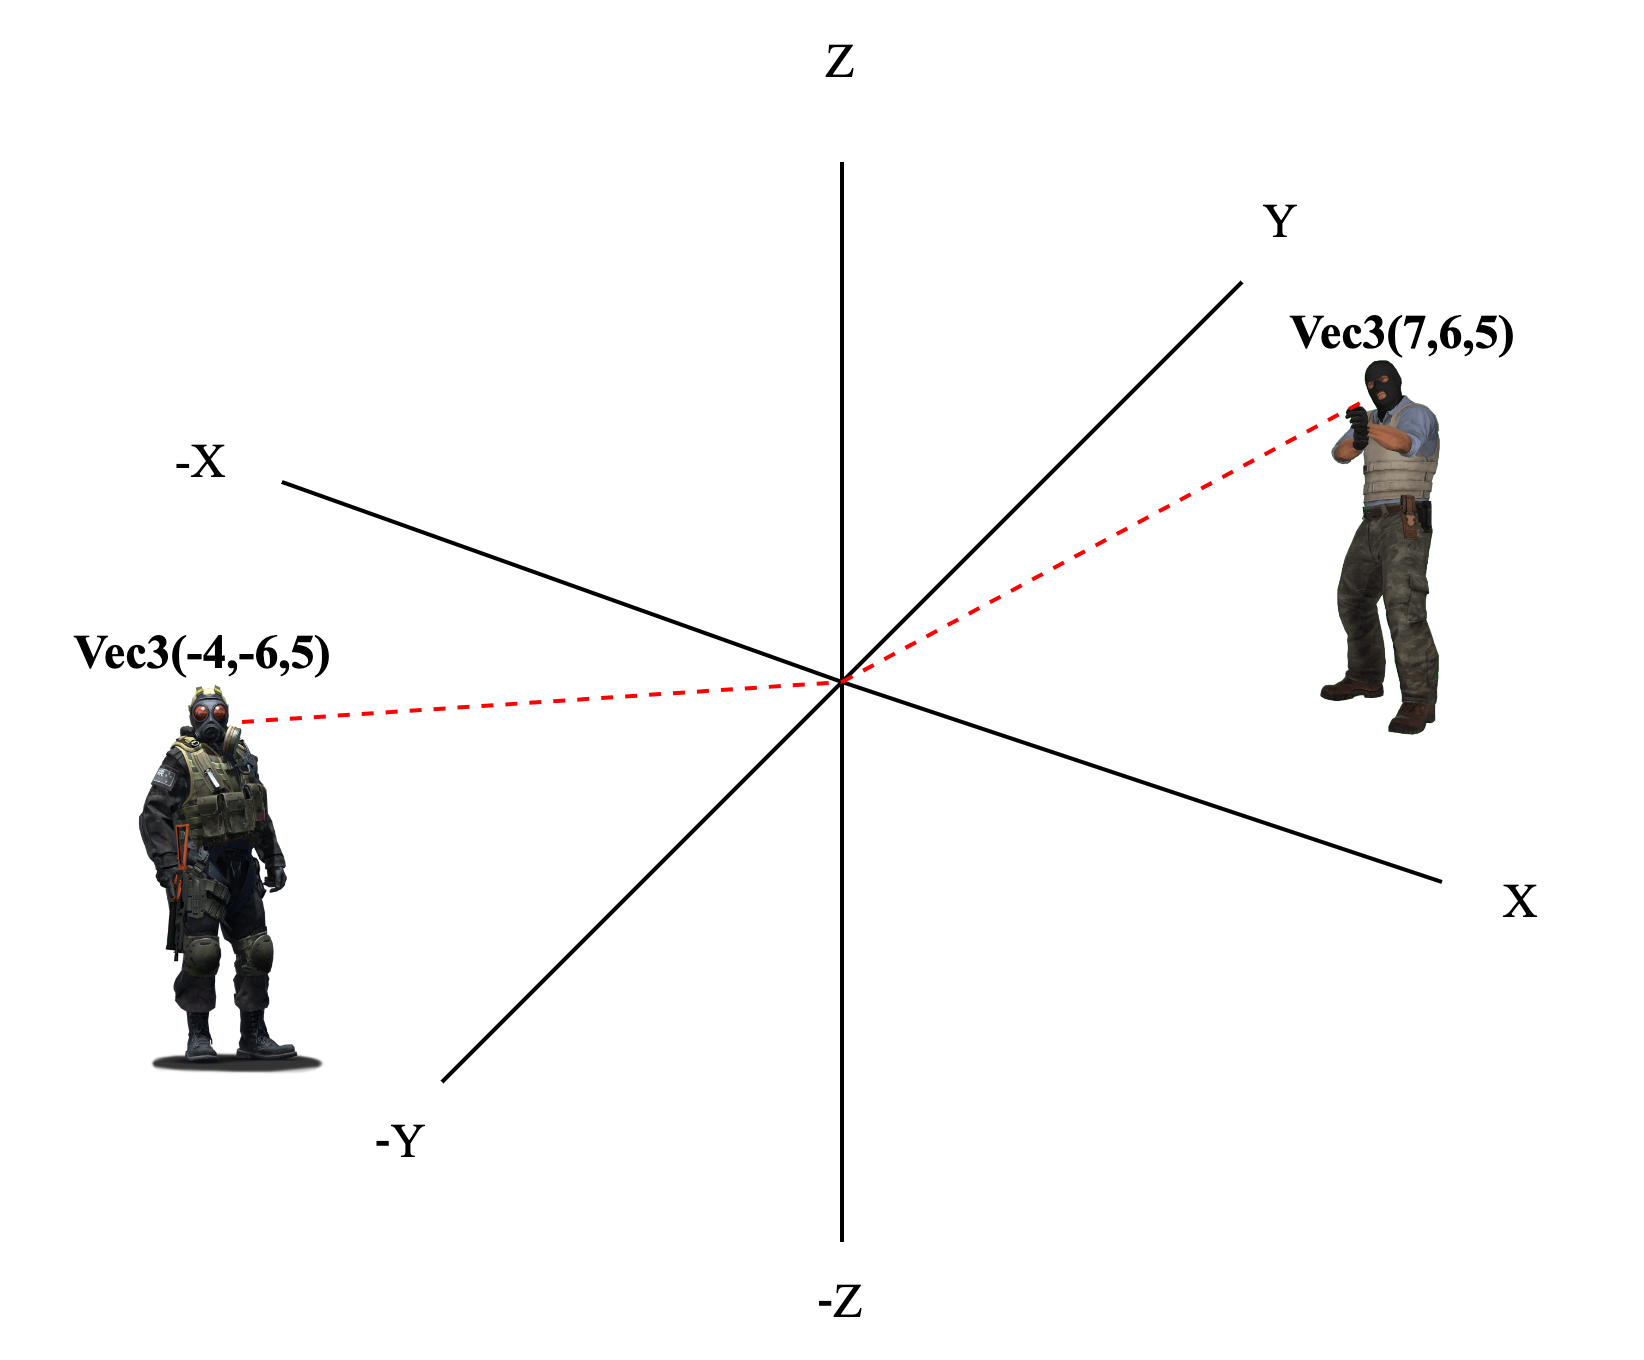
\includegraphics[width=0.75\linewidth]{images/Aimbot/Untitled Diagram.png}
    \caption{Representation of the player and enemy positions on the map.}
    \label{fig:player_enemy_positions}
\end{figure}

\subsubsection{Centering Coordinates on the Enemy}

To center the coordinate system on the enemy, we compute the relative position of the enemy with respect to the player by subtracting the player's position from the enemy's position:

\[
D = P_{\text{enemy}} - P_{\text{player}}
\]

Expressed in vector form:

\[
\mathbf{D} =
\begin{bmatrix} 
    x_{\text{enemy}} - x_{\text{player}} \\ 
    y_{\text{enemy}} - y_{\text{player}} \\ 
    z_{\text{enemy}} - z_{\text{player}} 
\end{bmatrix}
\]

This transformation ensures that the player’s position is effectively at the origin \((0,0,0)\), making it easier to compute aiming angles.

\begin{figure}[h!]
    \centering
    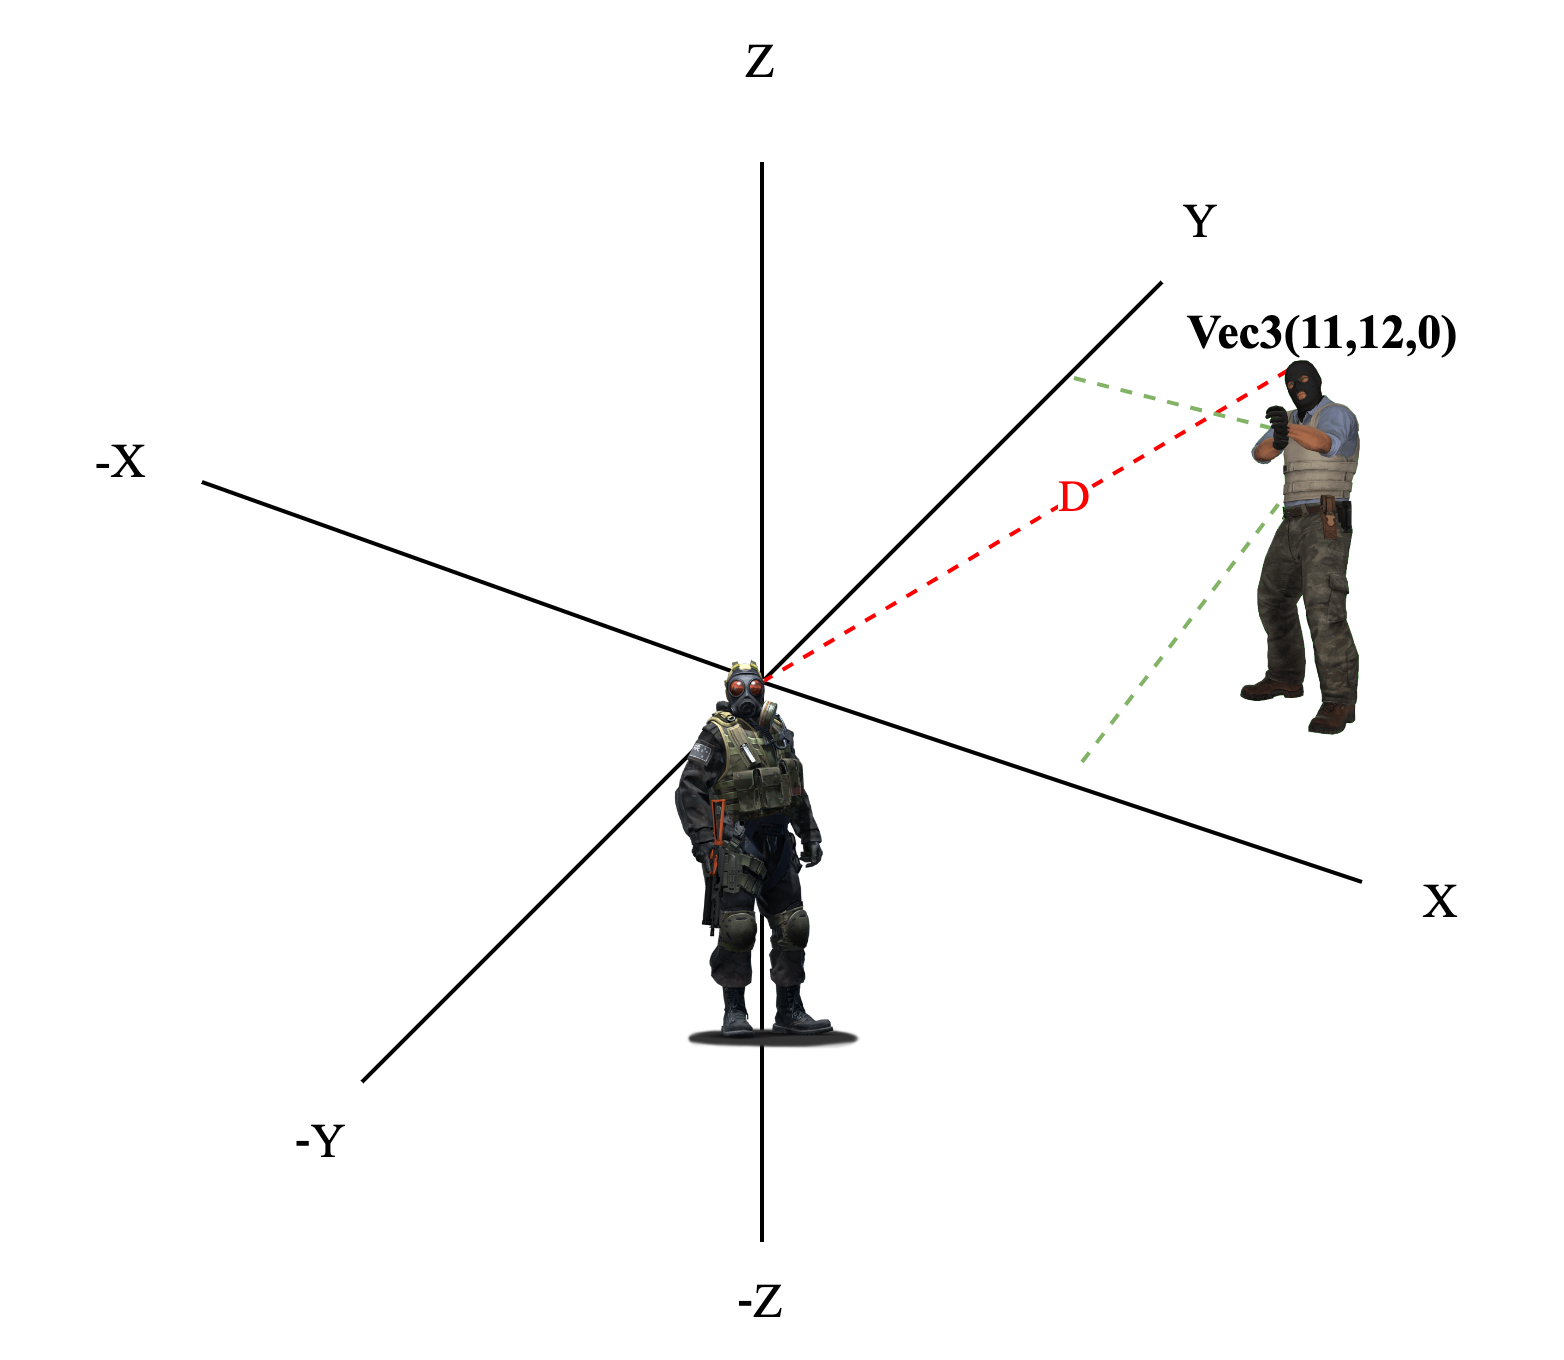
\includegraphics[width=0.75\linewidth]{images/Aimbot/Two.png}
    \caption{Computation of the displacement vector \( D \) from the player's eye to the target.}
    \label{fig:displacement_vector}
\end{figure}


\subsubsection{Local Coordinate System and Angle Calculation}

As illustrated in Figure~\ref{fig:direction_vector}, all calculations take place in a local coordinate system where the player’s eye position serves as the \textbf{origin}. The computed direction vector \( D \), depicted by the blue line, serves as the foundation for determining the required pitch and yaw adjustments.

\begin{figure}[h!]
    \centering
    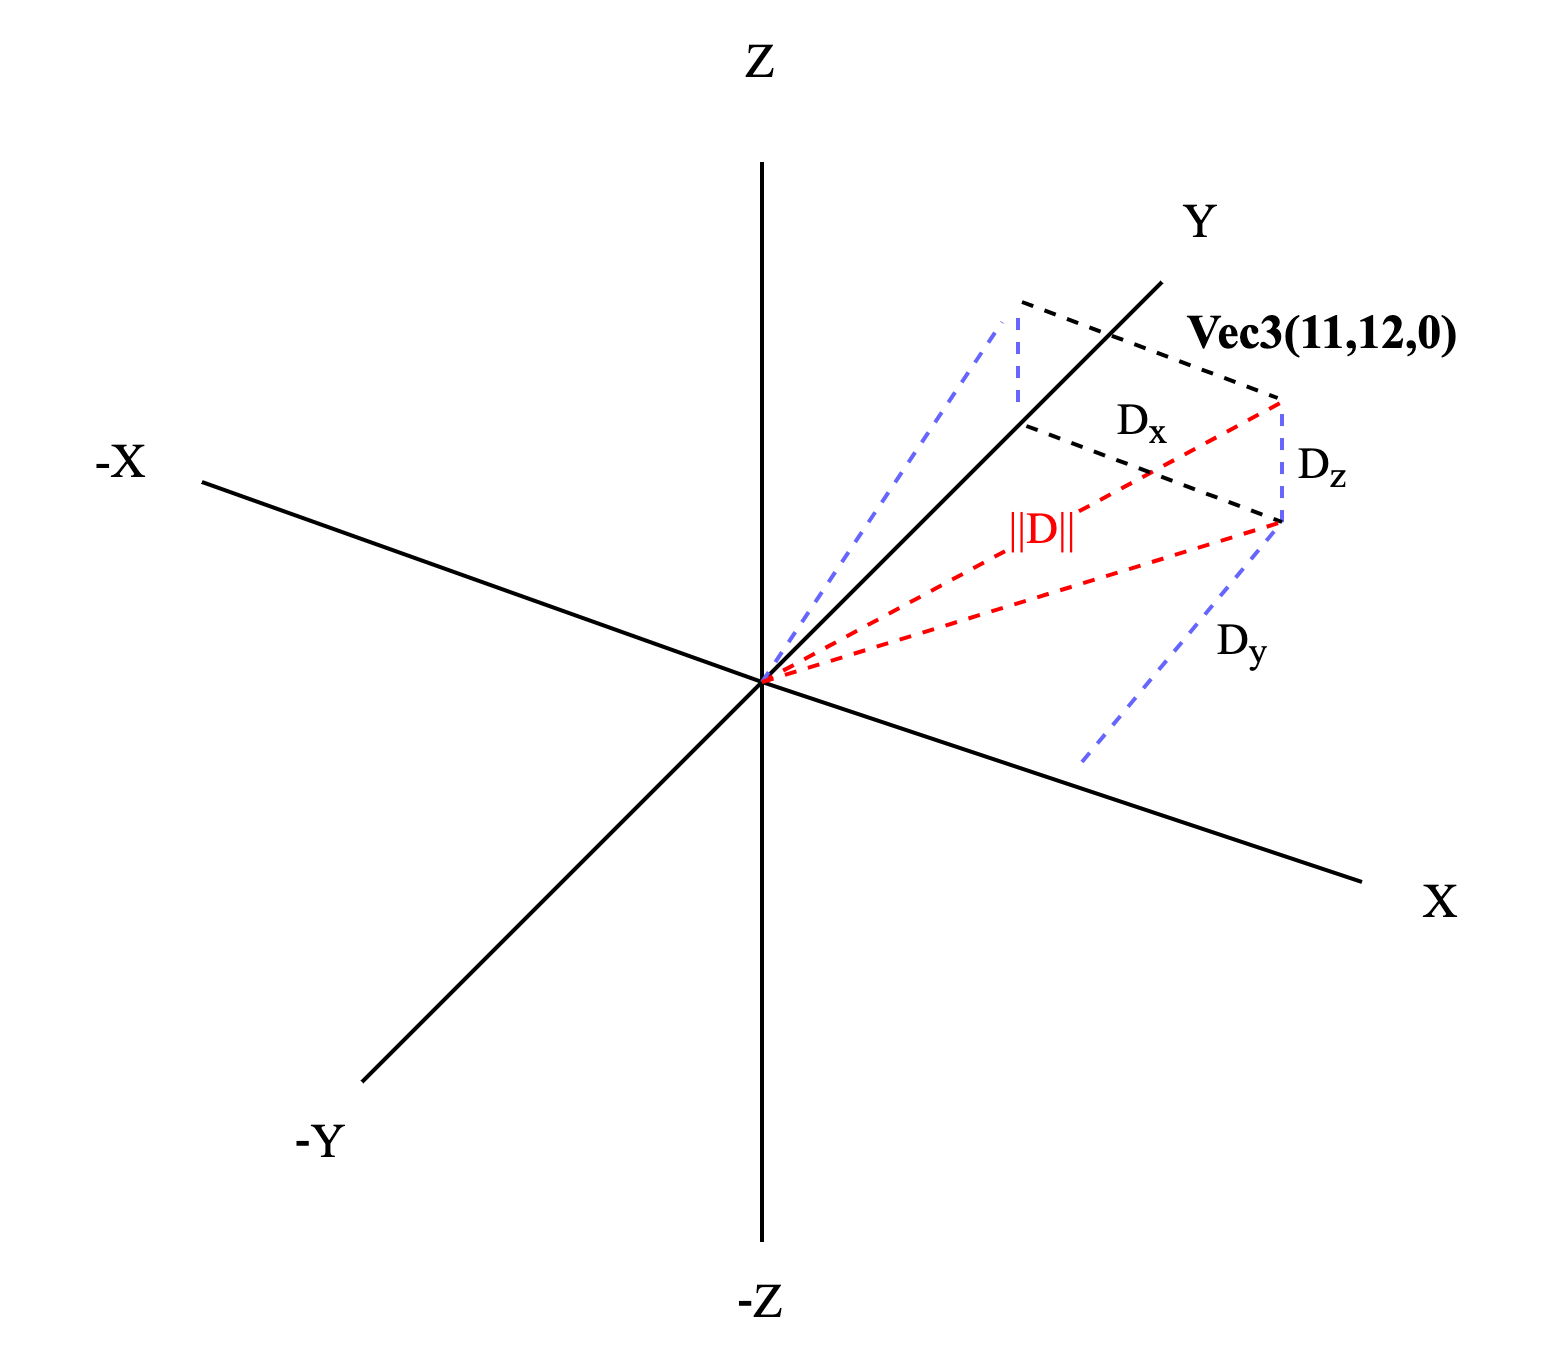
\includegraphics[width=0.75\linewidth]{images/Aimbot/Untitled Diagram(3).png}
    \caption{3D representation of the aiming direction vector.}
    \label{fig:direction_vector}
\end{figure}

This displacement vector is essential for calculating the angles necessary to adjust the player's aim. The yaw and pitch angles can be derived using trigonometric functions, which will be explored in the next section.


\subsubsection{Mathematical Computation of Aiming Angles}

Once the direction vector is obtained, the aimbot calculates the required \textbf{pitch} and \textbf{yaw} angles to align the player's crosshair with the target.

\paragraph{\textbf{Pitch Calculation} (\(\theta\))}  
The vertical adjustment necessary to match the enemy’s head height is determined by:

\[
\theta = \arcsin \left( \frac{D_z}{||D||} \right)
\]

where:

\[
||D|| = \sqrt{D_x^2 + D_y^2 + D_z^2}
\]

The \textbf{pitch} angle (\(\theta\)) is limited between \textit{\textbf{-90° and 90°}}, which corresponds to looking straight up or straight down.

\paragraph{\textbf{Yaw Calculation} (\(\phi\))}  
The horizontal adjustment required to rotate the player towards the enemy is calculated as:

\[
\phi = \arctan2(D_y, D_x)
\]

The function \(\arctan2(D_y, D_x)\) is used instead of \(\arctan(D_y / D_x)\) because it correctly determines the quadrant of the angle and prevents division errors when \( D_x = 0 \). The \textbf{yaw} angle (\(\phi\)) spans from \textit{\textbf{-180° to 180°}}, covering all possible directions.

\paragraph{\textbf{Angle Conversion:}}  
Since CS2 operates in degrees, a conversion from radians is necessary:

\[
\theta_{\text{degrees}} = \theta \times \frac{180}{\pi}, \quad
\phi_{\text{degrees}} = \phi \times \frac{180}{\pi}
\]



\subsection{Overwriting Player View Angles}

Once the aiming angles are computed, they must be applied to the player’s in-game camera. This is achieved by hooking into the game’s function responsible for setting view angles:

\begin{lstlisting}[style=cppstyle, caption={Overwriting Player View Angles}]
typedef void (__fastcall *SetViewAnglesFunction)(__int64 *a1, __int64 a2, Vec3 a3);
\end{lstlisting}

This function takes the following parameters:
\begin{itemize}
    \item A pointer to the player’s entity.
    \item An auxiliary parameter related to camera state.
    \item A vector \texttt{a3} containing the new pitch and yaw angles.
\end{itemize}

By injecting the computed angles into this function, the aimbot effectively reorients the player's view towards the target, ensuring near-instant alignment with minimal latency.

\subsection{Smoothing for Stealth}

To avoid detection by VAC, direct modifications to view angles are interpolated over multiple frames using a \textbf{smoothing algorithm}:

\[
\theta_{\text{new}} = \theta_{\text{current}} + \frac{(\theta_{\text{target}} - \theta_{\text{current}})}{S}
\]

\[
\phi_{\text{new}} = \phi_{\text{current}} + \frac{(\phi_{\text{target}} - \phi_{\text{current}})}{S}
\]

where \( S \) is the smoothing factor controlling transition speed. A larger smoothing value results in slower, human-like movements, significantly reducing the likelihood of detection.

By implementing smooth interpolation rather than instantaneously snapping to a target, the aimbot mimics natural aiming behaviors, thereby remaining undetected by VAC while maintaining effectiveness.

\newpage

\section{Bone Calculation: Extracting and Rendering Player Skeletons}

In this section, we describe how we extracted, visualized, and connected the bone structures used to animate player models in \textit{Counter-Strike 2}. These bones are essential for accurately representing player movement and orientation, and form the foundation for many ESP and aimbot features.

\subsection{Extracting Bone Data from Player Entities}

Each \texttt{PlayerPawn} entity in CS2 contains an internal memory structure that holds an array of bones. These bones represent all animation joints of the player model, from the pelvis and spine to the fingertips and eyes.

Through reverse engineering and memory analysis, we identified the layout of each bone entry in memory. Each bone follows the following structure:

\begin{lstlisting}[style=cppstyle, caption={Bone Memory Structure}]
class BoneData_t {
public:
    Vec3 vecPosition;           // 3D world-space position
    float flScale;              // Scale factor for animation
    Vector4D_t vecRotation;     // Rotation quaternion
};
\end{lstlisting}

This structure allows us to read the world-space position of each bone, which is later projected to screen coordinates for overlay rendering.

To access these bones, we enumerated all relevant bone indices used by terrorist player models. After extensive experimentation, we constructed a detailed enumeration mapping each bone to its corresponding index in memory. The following snippet presents a partial view of the enumeration:

\begin{lstlisting}[style=cppstyle, caption={Terrorist Bone Index Enumeration}]
namespace terroristBones {
    enum tBones : DWORD {
        pelvis = 0,
        spine_0 = 1,
        spine_1 = 2,
        spine_2 = 3,
        spine_3 = 4,
        neck_0 = 5,
        head_0 = 6,
        // ... continued through to:
        leg_upper_r_twist1 = 103
    };
}
\end{lstlisting}

This enumeration enables us to reference bones by name rather than raw index values, improving both readability and maintainability in our codebase.

\subsection{Visualizing Bone Indices on the Player Model}

After accessing the bone data, we developed a visualization tool to display each bone's index directly on the screen using our external overlay. This feature allows real-time debugging and inspection of the full bone structure.

\begin{figure}[h!]
    \centering
    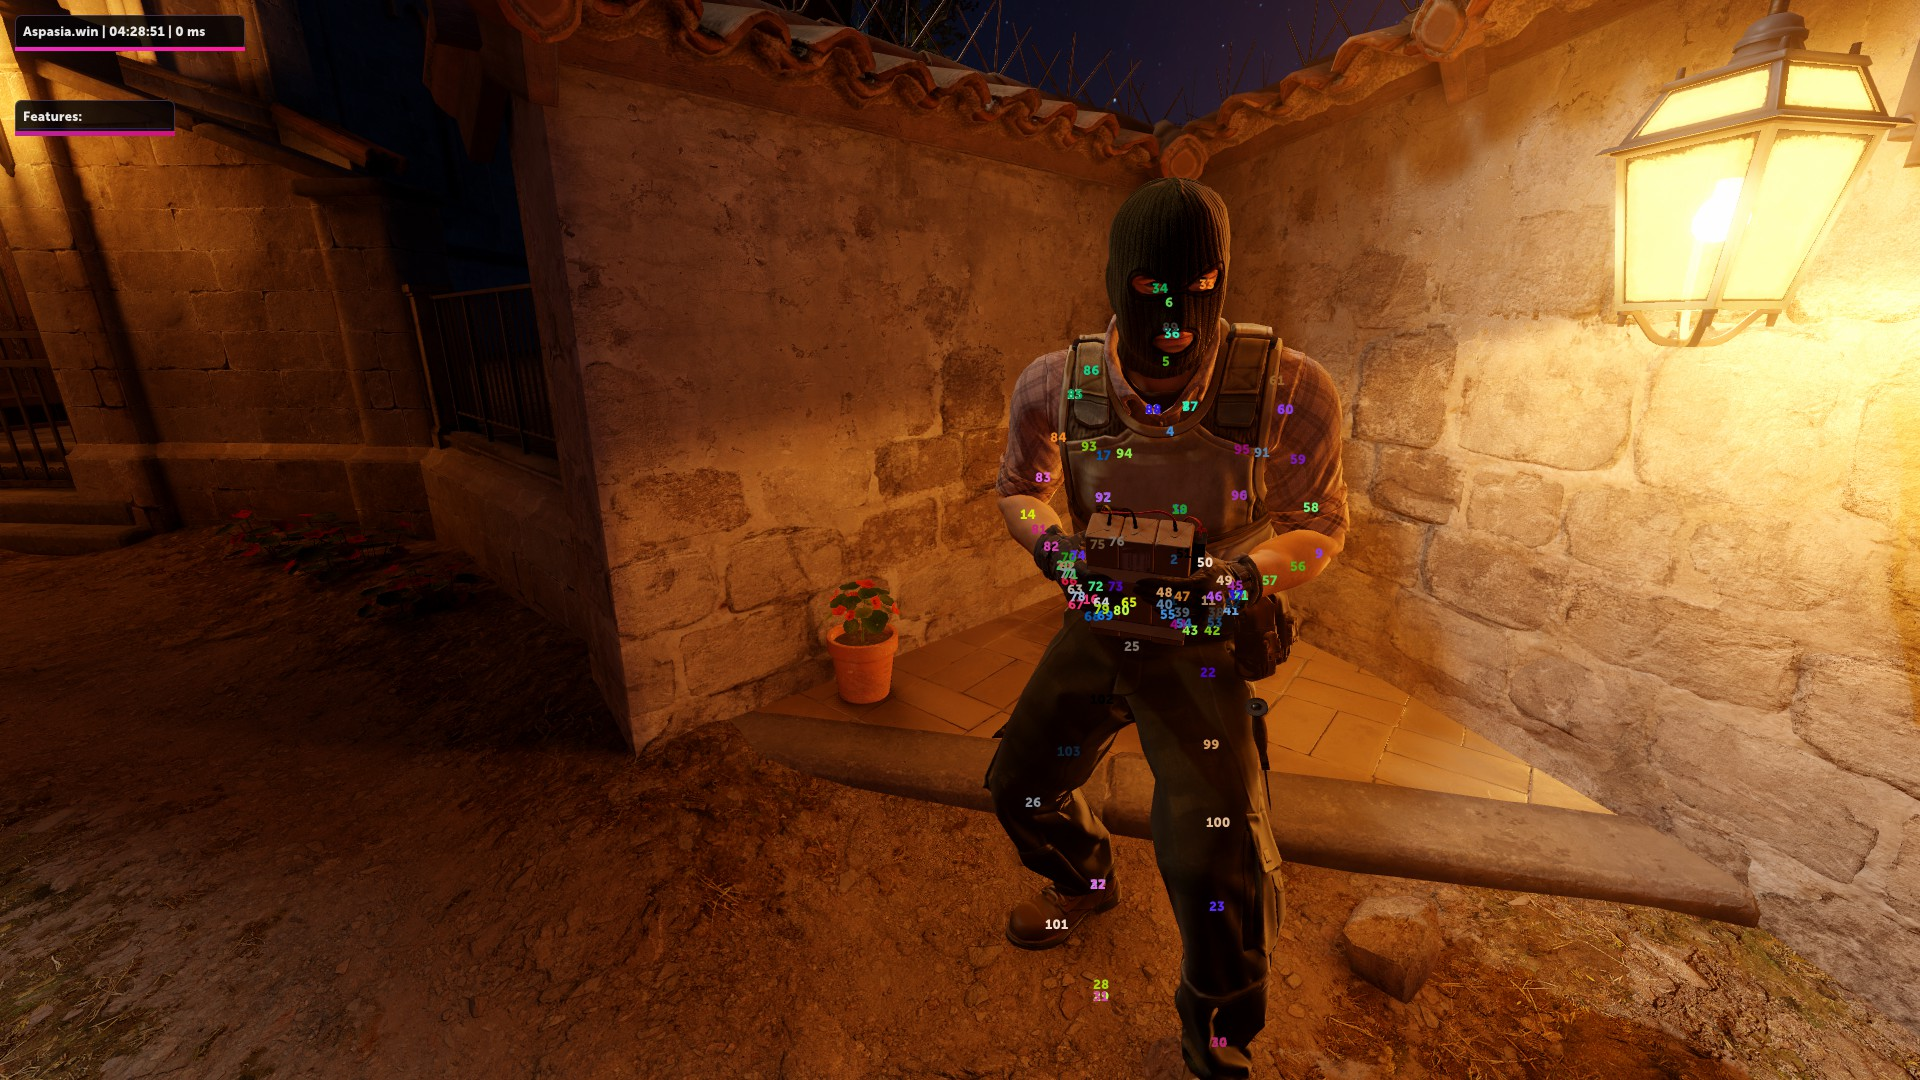
\includegraphics[width=0.8\linewidth]{images/Bones/730_22.jpg}
    \caption{Visualizing all bone indices rendered over the player model.}
    \label{fig:bone_debug}
\end{figure}

\begin{lstlisting}[style=cppstyle, caption={Displaying Bone Indices On-Screen}]
void RenderPlayerBones(C_PlayerPawn* player) {
    if (player == GetLocalPlayer()) return;

    for (int bone = terroristBones::pelvis; bone <= terroristBones::leg_upper_r_twist1; ++bone) {
        Vec3 worldPos = player->GetBone(bone)->vecPosition;
        Vec2 screenPos;

        if (!WorldToScreen(worldPos, screenPos)) continue;

        ImU32 color = IM_COL32((bone * 15) % 255, (bone * 35) % 255, (bone * 55) % 255, 255);
        DrawText(screenPos, std::to_string(bone).c_str(), color);
    }
}
\end{lstlisting}



This system projects each bone’s 3D position into 2D screen-space using the current game view matrix and renders its numeric index in a unique color. This was key for mapping bones during animation and ensuring accuracy in further rendering steps.

\subsection{Rendering a Connected Skeleton}

To enhance clarity and provide a meaningful representation of player posture, we implemented a simplified skeleton overlay. This system connects key bones with lines, forming a real-time stick-figure representation of the player’s body.

\begin{lstlisting}[style=cppstyle, caption={Drawing a Simplified Player Skeleton}]
void RenderSkeleton(C_PlayerPawn* player) {
    if (!player || player == GetLocalPlayer()) return;

    std::unordered_map<const char*, ImVec2> screenPos;
    for (auto& [name, index] : bones) {
        Vec3 world = player->GetBone(index)->vecPosition;
        Vec2 screen;
        if (WorldToScreen(world, screen)) {
            screenPos[name] = ImVec2(screen.x, screen.y);
        }
    }

    std::vector<std::pair<const char*, const char*>> links = {
        {"head", "neck"}, {"neck", "torso"}, {"torso", "pelvis"},
        {"torso", "left_clavicle"}, {"left_clavicle", "left_upper_arm"},
        {"left_upper_arm", "left_lower_arm"}, {"left_lower_arm", "left_hand"},
        . . .
        {"right_upper_leg", "right_lower_leg"}, {"right_lower_leg", "right_foot"}
    };

    for (auto& [a, b] : links) {
        if (screenPos.count(a) && screenPos.count(b)) {
            DrawLine(screenPos[a], screenPos[b], IM_COL32(255, 255, 255, 255), 2.0f);
        }
    }
}

\end{lstlisting}

This skeleton representation provides a clean and intuitive view of player pose and animation, aiding not only in cheat visualization but also in development of features such as aim prediction, hitbox tracing, and movement recognition.

\begin{figure}[h!]
    \centering
    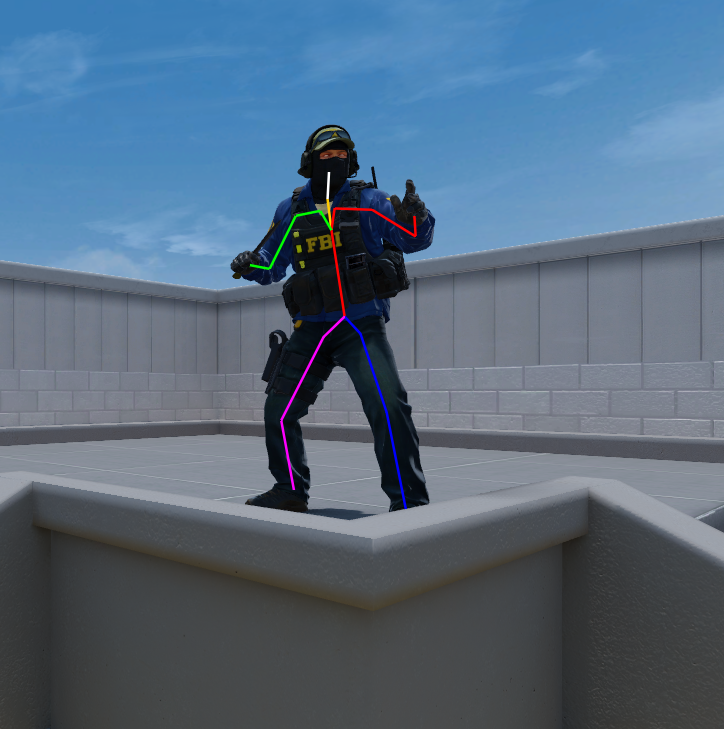
\includegraphics[width=0.8\linewidth]{images/imagen.png}
    \caption{Simplified player skeleton rendered using bone connections.}
    \label{fig:skeleton_overlay}
\end{figure}

\section{Anti-Aim: Misleading Enemy Targeting Systems}

Anti-Aim is a cheat technique designed to manipulate the visible orientation of a player’s model in order to confuse enemy aimbots and reduce the likelihood of being hit in combat. Rather than improving offensive capabilities like an aimbot or triggerbot, Anti-Aim provides a defensive advantage by making it significantly harder for both human players and automated cheats to land accurate shots.

\subsection{What Is Anti-Aim?}

In \textit{Counter-Strike 2}, a player's view direction is broadcast to the server and other clients to render the model's orientation. Normally, this direction reflects where the player is actually looking and aiming. Anti-Aim breaks this consistency by desynchronizing the player's real viewing direction from the one seen by others. As a result, opponents and external cheats perceive the cheater as facing in the wrong direction, leading them to aim at incorrect hitboxes.

This desynchronization creates an illusion where, for example, the cheater may be looking forward from their own perspective, but appear to be looking sideways or even backwards to others. Since many cheats rely on model orientation to predict aim points, this strategy effectively disrupts their logic.

\subsection{Types of Anti-Aim}

There are several ways Anti-Aim can be implemented, each with different goals such as stealth, aggressiveness, or maximum desync:

\begin{itemize}
    \item \textbf{Fake Yaw (Yaw Desync):} The player's view direction (yaw angle) is faked to appear offset from their real direction. This is the most common and effective form of Anti-Aim.
    
    \item \textbf{Pitch Exploits:} Sends pitch values that are outside the game's allowed viewing range (e.g., looking completely up or down), which causes visual glitches in the player model. This can result in the head being rendered inside the chest or legs, making headshots harder.
    
    \item \textbf{Yaw Jitter:} Rapidly switches between multiple fake yaw angles, making the model “shake” or spin unpredictably. While easy to spot visually, this is highly effective against poorly written aimbots.
    
    \item \textbf{Spinbot:} Continuously rotates the model in a full 360° loop at high speed. This guarantees total desync but is highly obvious and generally used in rage hacking contexts rather than legit cheating.
    
    \item \textbf{Static Desync:} Applies a fixed yaw offset to the model, making the cheater appear to always be looking in a different direction. This is more subtle and used in “legit” cheating configurations.
\end{itemize}

\subsection{Lower Body Yaw (LBY) and the LBY Breaker}

In older Source-based games like CS:GO, the engine separated the upper and lower body yaw (LBY) values for animation purposes. LBY would only update under specific conditions, such as when a player stopped moving. Exploiting this timing, cheaters could delay the LBY update and create a temporary desynchronization window between the real view angles and the visible model. This method was known as the \textbf{LBY Breaker}.

While CS2’s Source 2 engine has changed animation handling, similar concepts still apply. Some anti-aim techniques attempt to delay animation state updates or force inconsistent transitions to create fake angles, although LBY is no longer exposed in the same way. Nonetheless, the idea of exploiting animation update delays remains an active area in cheat development.

\subsection{Benefits for the Cheater}

Anti-Aim provides several key advantages:

\begin{itemize}
    \item \textbf{Aimbot Evasion:} Many aimbots target the visible model's head or chest hitbox based on predicted angles. Anti-Aim misaligns these predictions, causing the aimbot to miss entirely.
    
    \item \textbf{Confusing Human Opponents:} Players may struggle to read movement or pre-aim accurately when the enemy model behaves unpredictably or appears to be looking away.
    
    \item \textbf{Reduced Headshot Risk:} By forcing the head into glitched positions (e.g., inside the torso), it becomes harder to land critical hits, especially for players relying on flick shots or crosshair placement.
    
    \item \textbf{Overwatch Safety:} When configured subtly, Anti-Aim can provide these benefits without looking suspicious in demos, reducing the risk of bans from human reviewers.
\end{itemize}

\subsection{Importance in Modern Cheats}

Anti-Aim has become one of the most essential components in competitive cheat configurations, especially in cheat-vs-cheat environments (e.g., HvH—Hack vs. Hack matches). In such scenarios, defensive capabilities are as important as offensive ones, and the ability to evade incoming fire becomes a major strategic advantage.

Furthermore, as anti-cheat systems become more advanced in detecting aimbots and wallhacks, subtle and effective Anti-Aim techniques provide cheaters with a low-profile method to gain survivability without triggering automated bans.






\newpage
\newpage
\newpage
\newpage




